\documentclass[thesis.tex]{subfiles}
\begin{document}
\chapter{Introduction}
\label{chap:introduction}


% An image right here at the top can look really cool!

%\section{Problem}
%Modern economy relies heavily on steady production of energy. Traditional energy sources mostly include non-renewable energy like coal, natural gas and fossil-fuel-based power plants. They are highly reliable and predictable in nature as the output can be moderated according to the consumers’ requirements. However, they are increasingly undesirable due to their adverse environmental impacts.\\\\
%Germany’s Renewable Energy Sources Act or EEG (German: Erneuerbare-Energien-Gesetz)\cite{deuterneu} is a series of legislations introduced in 2000 aimed at encouraging development of renewable energy sources (RES) such as wind and solar energy. As of 2017, RES constitute nearly 36.2\% of gross electricity consumption and the target is to meet over 50\% of the production by 2030\cite{deuterneu}. The inclination towards RES is due to their non-existent or low toxic emissions and inexhaustibility. However, inclusion of RES into the national power grid for energy production adds to grid’s volatility as such sources’ outputs cannot be controlled and depend on the on-site meteorological conditions at any given time. Therefore, this increased dynamicity of the grid mandates a higher monitoring resolution for safe grid operation. \\\\
Introduced by Fred Schweppe\cite{Schweppe} in 1969, the system state of electrical power systems can be defined as the vector of steady-state complex voltages, i.e. magnitudes and angles at the buses of the network. He defined state estimation (SE) in power systems as “a data processing algorithm for converting redundant meter readings and other available information into an estimate of the state of an electric power system"\cite{Schweppe}. Once the system state is computed, every other electrical quantity including those which are not telemetered or those which are missing can be easily calculated. In other words, SE in power grids acts as the process for extracting reliable information from noisy measurement data obtained from sensors and measuring devices placed throughout the grid and allows to determine all other relevant quantities. This information is crucial in avoiding potential emergencies, resolving an existing emergency or recuperating from an emergency\cite{Liacco}. Hence, SE is indispensable for the rest of the energy management system (EMS) components.\\\\
Considering Germany’s ambitious renewable energy targets and the state of increasingly large current RES infrastructure and its dynamicity, SE is increasingly required to readily respond to grid voltage fluctuations. However, the major hurdles against obtaining a higher monitoring time resolution through SE over a vast nationwide power grid are currently the required large computational power and correspondingly long execution times. \\\\

\section{Motivation}
In order to achieve a higher SE resolution for a large power system, it is necessary to find ways to accelerate the process of SE. Two potential solutions investigated in the thesis are listed below:
\begin{enumerate}
	\item Efficient computations using manycore GPGPU processors\cite{KarimipourAcc}.
	\item Partitioning of the original problem into smaller subproblems for reduced computational burden\cite{Xiong}\cite{Muscas}\cite{KarimipourDec}.
\end{enumerate}
General Purpose computation on Graphics Processing Unit (GPGPU) refers to the use of a graphics processing units (GPU) for calculations beyond its original scope of tasks. GPU are ‘massively parallel’ in nature because of their ability to launch and run a vast number of threads concurrently resulting in remarkably high arithmetic throughput.\\\\
GPGPU provides the potential to accelerate the problem of SE due to the presence of various large matrix-matrix and matrix-vector operations that can be expressed as data-parallel computations on GPU. The data-parallel implementation of the solution is capable of delivering significantly higher throughputs on a GPU with varying accuracies based on the floating-point precisions used. Hence, through porting of the serial SE algorithm to the GPU to exploit its high degree of parallelism, a higher monitoring resolution can be obtained.\\\\
Similarly, another potential approach to accelerate the SE computation can be through decentralization of power grids which is based on divide-and-conquer strategy. In this approach, the original SE problem is split into many smaller subproblems. This implies that the power grid can be broken down into smaller balanced partitions or sub-areas as shown in the Figure~\ref{fig:subareas}. 

\begin{figure}[H]
	\centering
	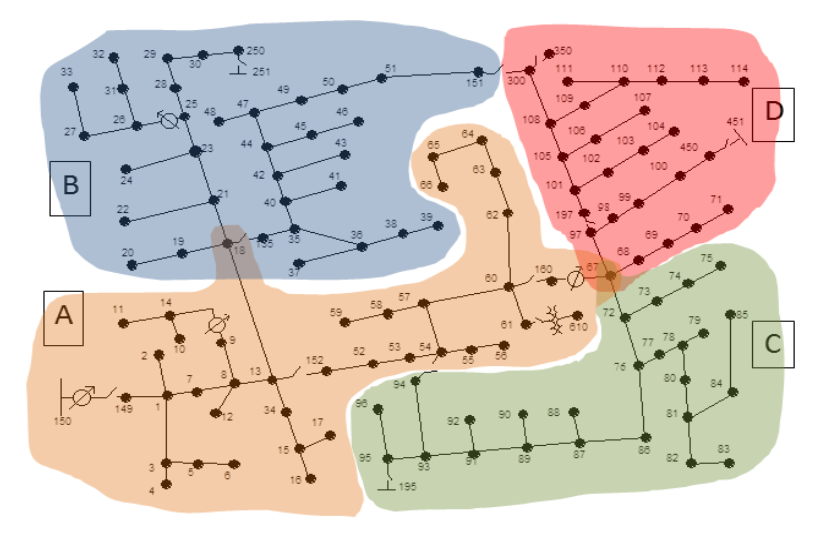
\includegraphics[scale=0.6]{sub-areas}
	\caption{IEEE 123-bus test network: organization in sub-areas~\cite{Muscas}}.
	\label{fig:subareas}
\end{figure}

The local system states of each sub-area can be calculated with lower amount of resources and potentially less time through distribution of computational burden to separate threads or processes. The reduction in computational burden is mainly due to a decrease in the order of the matrices involved. The global system state can be then computed through a fast recombination of the local results by exploiting interface information and with minimum possible recombination error. \\\\
Combining the above two approaches, performing decentralized SE on GPUs offers acceleration of manycore processors alongside distribution of computational burden. In this thesis, the performance and accuracies of SE on decentralized power grids are investigated using the supported floating-point precisions and its limitations are presented. 


\section{Contributions of the Thesis} \label{bib:goals}
\begin{enumerate}
	\item The possible approaches to port serial SE algorithm to a suitable GPGPU platform are presented along with their advantages and disadvantages. CUDA is a widely-accepted GPGPU platform for the given purpose. A CUDA-accelerated solution is prepared that operates in single and double precision modes.
	\item The performance and accuracy of the CUDA-accelerated application operating with different precisions are analyzed against the reference serial SE algorithm. It is expected that different precisions introduce varying magnitudes of errors in the final result. Alongside high efficiency, low errors are desirable.
	%\item An experimental approach to generate large power systems and subsequent grid-decentralization is developed. Power grids with hundreds or thousands of busses can be generated using this technique and readily partitioned into sub-areas.
	\item The performances and accuracies of decentralized SE for various grid sizes are compared to the centralized SE to justify the usability of GPGPU in decentralized SE alongside related limitations. GPUs with different architectures and arithmetic throughputs are used to gather the performance metrics and present the findings.
\end{enumerate}


\section{Thesis Outline}
%Describe the structure of this document.

%Next chapter ....
%\\
%\autoref{chap:prevwork} discusses ...
%\\
%Our own contribution ... described in \autoref{chap:basics}.
%Results are evaluated and discussed in \autoref{chap:eva}.
%\\
%Finally, \autoref{chap:concl} will summarize the thesis and give an outlook to possible future work.
The thesis is categorized into 7 chapters as follows: \\
\begin{itemize}
	\item Chapter \ref{chap:introduction} provides a detailed introduction to the problem and a motivation to solve the stated problem. It listed out the goals of the thesis and clearly states the main contribution produced from this work.
	\item Chapter \ref{chap:preq} deals with foundations in SE in power systems, IEEE 754 floating-point representations and NVIDIA’s parallel computing platform called CUDA.
	\item Chapter \ref{chap:prevwork} discusses the state of the art in CUDA-accelerated SE and power-grid decentralization. This section takes into consideration the findings published in a number of verified papers and journals by various researchers working in analogous domains.
	\item Chapter \ref{chap:concept} provides the details concept that would be used to build a proof-of-concept application to test our hypothesis.
	\item Chapter \ref{chap:implementation} presents the implementation details of the aforementioned application using various diagrams. It discusses the pertinent software architecture along programming techniques and algorithms.
	\item Chapter \ref{chap:eva} discusses the evaluation of the proof-of-concept application against test data from various grid-sizes and significance of the results obtained through the experiments performed.
	\item Chapter \ref{chap:concl} summarizes the findings and limitations in conclusion. It also provides the possible future works that can be carried out to take the topic forward.
\end{itemize}


\subfilebib % Makes bibliography available when compiling as subfile
\end{document}